\documentclass{IOS-Book-Article}
\usepackage{mathptmx}
\usepackage{comment}
\usepackage{graphicx}
\graphicspath{ {./figures/} }
\usepackage{subfig}
%\usepackage{times}
%\normalfont
%\usepackage[T1]{fontenc}
%\usepackage[mtplusscr,mtbold]{mathtime}
%
\begin{document}
\begin{frontmatter}              % The preamble begins here.
%\pretitle{Pretitle}
\title{Machine Learning Assisted Citation
 Screening for Systematic Reviews}
\runningtitle{IOS Press Style Sample}
%\subtitle{Subtitle}
%
\author[A]{\fnms{Anjani} \snm{Dhrangadhariya}%
\thanks{Corresponding Author: Anjani Dhrangadhariya, University of Applied Sciences Western Switzerland (HES-SO), Technopole 3,
3960 Sierre, Switzerland; E-mail:
anjani.dhrangadhariya@hevs.ch.}},
\author[B]{\fnms{Roger} \snm{Hilfiker}}
,
\author[A]{\fnms{Roger} \snm{Schaer}}
and
\author[A,C]{\fnms{Henning} \snm{M\"uller}}
%
\runningauthor{B.P. Manager et al.}
\address[A]{University of Applied Sciences Western Switzerland (HES-SO), Sierre, Switzerland}
\address[B]{School of Health Sciences, HES-SO Valais-Wallis, Leukerbad, Switzerland}
\address[C]{University of Geneva (UNIGE), Geneva, 
 Switzerland}
%
\begin{abstract}
Evidence-based practice is highly dependent upon up-to-date systematic reviews (SR) for decision making.
However, conducting and updating systematic reviews, especially the citation screening for identification of relevant studies, requires much human work and is therefore expensive.
Automating citation screening using machine learning (ML) based approaches can reduce cost and labor.
Machine learning has been applied to automate citation screening but not for the SRs with very narrow research questions.
This paper reports the results and observations for an ongoing research that aims to automate citation screening for SRs with narrow research questions using machine learning.
The research also sheds light on the problem of class imbalance and class overlap on the performance of ML classifiers when applied to SRs with narrow research questions.
\end{abstract}
%
\begin{keyword}
Systematic reviews, Automation, Natural language processing, Machine learning
\end{keyword}
\end{frontmatter}
%
\thispagestyle{empty}
\pagestyle{empty}
%
\section{Introduction}
%
% The problem
Summarizing evidence in a specific domain through the process of conducting systematic reviews (SR) becomes increasingly difficult with an exponential increase in the number of primary research publications and an increasing variety of publishers.
With this increased publication-rate, citation screening for conducting the SRs has become  time-consuming and labour intensive.
The core of citation screening involves manually categorizing the studies found in literature search into relevant or non-relevant depending upon predefined criteria for the research question at hand~\cite{cochraneHandbook}.
This screening is usually performed by two independent reviewers, who often can not keep up with the manual process of screening the studies and constantly updating outdated SRs~\cite{pmid22587960}.

% Background
In the area of physiotherapy and rehabilitation such an exponential increase in the number of publications is also observed\footnote{https://www.ncbi.nlm.nih.gov/pubmed?term=(physiotherapy)\%20OR\%20rehabilitation}.
For an ongoing review on exercise and non-exercise interventions in reducing cancer-related fatigue retrieved over 30,000 references, about 2,000 of which were published in 2017 alone. It took more than 200 hours each for the two independent reviewers to manually assess the titles and abstracts for relevance to the research question before the studies were taken for further meta-analysis~\cite{Hilfiker651}.

% Our solution
%Manual citation screening of the searched studies is the process of classifying these studies into relevant vs. non-relevant regarding the chosen criteria.
Supervised machine learning based classification approaches are successfully applied for automation of citation screening but either only for broad and shallow SRs~\cite{pmid30646959} or SRs that retrieved fewer than 6,000 studies~\cite{Lerner2019-tj}.
However, there are SRs that address very specific research questions leading to narrow, predefined criteria for selection of relevant studies to be included for meta-analysis.
For such narrow SRs, inclusion prevalence becomes as low as 10\%, which means that out of all the studies retrieved during the search phase, 90\% are excluded as non-relevant.
A narrow research question combined with a low inclusion prevalence leads to class imbalance and class overlap problems for classification tasks that generally reduce classifier performance~\cite{Garcia2006-wn}.
Class overlap cannot be artificially controlled but class imbalance can be tackled using oversampling or undersampling~\cite{pmid25738806}.
%which aim to bring the number of instances in the minority class equal to the number of instances in the majority class.
In this work, we aim to explore machine learning and natural language processing to assist citation screening in SRs with a narrow research question and low inclusion prevalence using word embeddings and random oversampling.
%
\section{Methods}
%
\subsection{Datasets}
%
Data sets from the open access literature were used in the work described here.
% Dataset used to generate word embeddings
%
\paragraph{Word embedding}
\label{method:dataset_embedding}
% (255 million words) 
Titles and abstracts (TA) of 2.09 million studies included in the PubMed Central Open-Access subset (PMC-OA) were used to generate semantic word embedding using the two most common architectures: word2vec and  fastText~\cite{word2vec, bojanowski2017enriching}.
% Dataset used for experimentation
%
\paragraph{Data for the screening process}
\label{sysrev_dataset}
%
The data set used to test automation approaches included the studies identified for citation screening in an update to the systematic review by Hilfiker \textit{et al.}~\cite{Hilfiker651}. % Roger: here you should write that this was from an update of reference Hilfiker651, not this study itself.
The data set included TA from 31,279 studies identified during the search phase of this SR.
These studies were already manually assessed for relevance and labelled by two reviewers into two mutually exclusive labels.
4,066 studies assessed as relevant were labelled ``include" and
%27,213 studies assessed as non-relevant were labelled ``exclude".
the rest were labelled ``exclude".
The inclusion prevalence for this case is only about 13\% leading to class imbalance.
%
\subsection{Screening Automation}
%
To automate the screening and explore the effect of class imbalance, six supervised binary classifiers were trained to classify documents into ``include" (relevant) vs. ``exclude" (non-relevant) using the data set of Section~\ref{sysrev_dataset} represented using corpus-specific static word embedding.
This approach follows steps enumerated below.
%This approach follows the listed steps: 1) Generation of word embedding, 2) Dataset and text preprocessing, 3) Random oversampling, 4) Feature extraction, and 5) Classifier training and evaluation.
%
\paragraph{1. Word embedding generation}
%
To generate embedding, the PMC-OA data were lower-cased and all punctuation except the hyphens were removed.
% Reviewer_comment reviewer 2: Added some methodological details
Phrase generation was then performed using the word2phrase tool\footnote{https://github.com/travisbrady/word2phrase} to identify frequently occurring bi-grams.
The output of phrase generation along with the unigrams was fed to gensim's word2vec\footnote{https://radimrehurek.com/gensim/models/word2vec.html} and to fastText\footnote{https://radimrehurek.com/gensim/models/fasttext.html} using the hyperparamters in Table~\ref{table:1} to obtain two dense, semantic, real-valued word embeddings~\cite{Goldberg2015-qv}.
%
\vspace{1em}
\begin{table}[h!]
\centering
\begin{tabular}{p{1.5cm}p{1cm}p{1.5cm}p{1cm}p{1.5cm}p{1cm}  }
 Parameter & Value & Parameter & value & Parameter & value\\
 \hline
 Size   & 300    & Alpha &   0.05 & bucket* & 2000000\\
 Window & 5  & min\_alpha   & 0.0001 & minn* & 3\\
 min\_count  & 5 & sample  &  0.0001 & maxn*   & 6 \\
 sg & 1 & iter/ epoch &  5 & seed & 1\\
 hs & 1  & negative & 5 & & \\ 
 \hline
\end{tabular}
\vspace{1em}
\caption{Hyperparameter values used to generate word embeddings using gensim's word2vec and the fastText functionality. (*) means that these parameters were available only for the fastText embeddings.}
\label{table:1}
\end{table}
%
\paragraph{2. Data set for text pre-processing}
\label{method:preprocessing}
%
Post deduplication and removal of non-English language studies led to 25,540 studies remaining.
For these remaining studies, the text was lower-cased and tokenized into words using NLTK\footnote{https://www.nltk.org/api/nltk.tokenize.html} (Natural Langauge ToolKit).
Irrelevant tokens were removed using a predefined set of stop-words provided by NLTK and PubMed\footnote{https://www.ncbi.nlm.nih.gov/books/NBK3827/table/pubmedhelp.T.stopwords/}.
%Stop-words were removed using a predefined set of words provided by NLTK, PubMed\footnote{https://www.ncbi.nlm.nih.gov/books/NBK3827/table/pubmedhelp.T.stopwords/}, and corpus-specific stop-words identified during the experiments. 
Additional corpus-specific stop-words identified during the experiments with the training set were removed accordingly. 
The text normalization process converted British English terms into American English.
After token lemmatization, a corpus vocabulary was constructed from all the unique unigram and bigram tokens. 
To scale this vocabulary down, uninformative short tokens with fewer than five characters and the tokens with vocabulary count lower than five were removed assuming they were not representative of the classes.
%
\paragraph{3. Random oversampling}
\label{method:oversampling}
%
Class imbalance often deteriorates the classifier performance, so in the present data set it was addressed using naive random oversampling.
This method randomly duplicates data points from the minority class and brings the total number of instances in the minority class equal to the majority class~\cite{Garcia2006-wn}.
%
\paragraph{4. Feature extraction}
\label{method:feature_extraction}
%
Feature extraction was performed to generate real-valued, dense feature vectors from text.
%% Reviewer_comment reviewer 1:  What are the exact input data and 
These features were used as input to train the supervised ML classifiers.
For non-neural ML classifiers, from each of the 25,540 studies word vectors were extracted for each token using both generated word embeddings.
All vectors for each token in the individual study were averaged over the entire study normalized by study length to produce a single 300-dimensional vector representing a particular study.
For the Convolutional Neural Network (CNN), feature extraction was part of the model, where a static, non-trainable weight matrix generated from the word embedding was provided with the embedding layer to extract token word vectors during training.
%
\paragraph{5. Classifier training and evaluation}
\label{method:cpe}
%
Six classifiers including Logistic Regression (LR), Support Vector Machines (SVM), k-nearest neighbour (KNN), Decision Trees-CART (DT), Random Forest (RF), and CNNs were trained and evaluated over the generated text feature to perform binary classification.
Hyperparameter tuning was performed using GridSearch.
A CNN was trained using hyperparamters loosely based on suggestions from Zhang \textit{et al.}~\cite{Zhang2015-qd}.
%  Reviewer_comment reviewer 1: What are the exact input data and what are the output data?
%Estimated probabilities for whether a study belonged to class ``include" or not are output by all the classifiers.
Classifier performance before and after oversampling was evaluated on an unseen validation data set and metrics pertinent to imbalanced classification like precision, recall, F1 and precision-recall AUC (PR-AUC) score were tracked~\cite{pmid25738806}.
%
\section{Results and Discussion}
%
%\subsection{Dataset representation}
The data set used for training and evaluating the classifiers comprised 2,259 relevant studies labelled ``include" and 23,281 labelled ``exclude".
Cosine similarity between class centroid vectors for the ``include" and ``exclude" classes before and after oversampling is 0.985814 and 0.985824 respectively.
A high cosine similarity is indicative of high class overlap even after tackling the class imbalance using oversampling (see Figure~\ref{fig:tsne}).
%The dataset vocabulary coverage for both the word embeddings was 60.629\%.
%
\begin{figure}%
    \centering
    \subfloat{{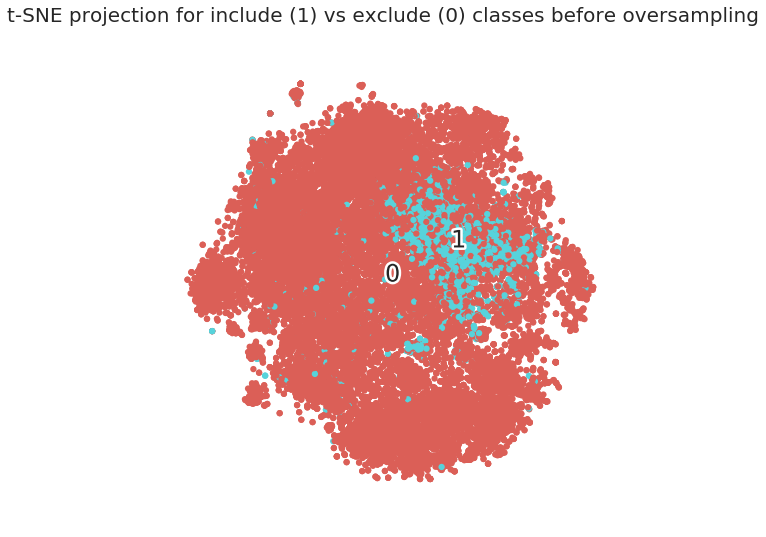
\includegraphics[width=5.12cm]{tsne_include_exclude} }}
    \qquad
    \subfloat{{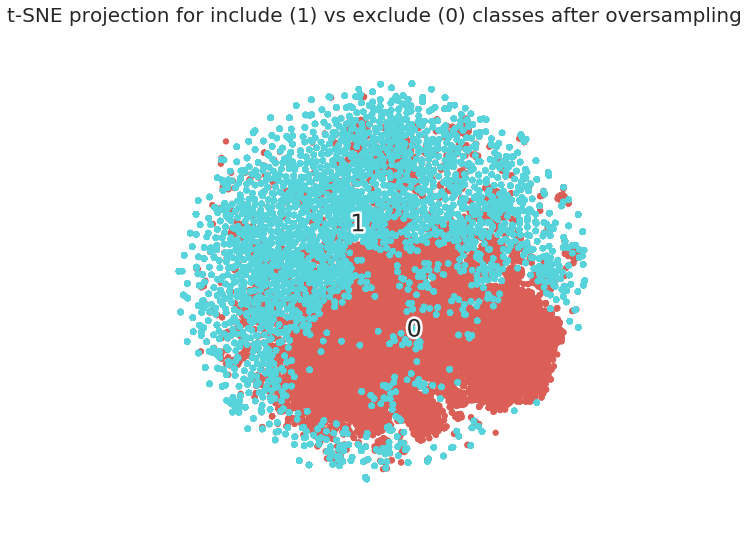
\includegraphics[width=5cm]{tsne_include_exclude_oversampling} }}
    \caption{A t-SNE projection for 25,540 studies labelled ``include" vs. ``exclude" before and after oversampling.}%
    \label{fig:tsne}
\end{figure}
%\subsection{Classifier performance and evaluation}

The results obtained by applying classifiers on the data set before and after random oversampling are summarized in Table~\ref{tab2:no_oversampling} and \ref{tab3:oversampling}.
Before oversampling, the classifiers focused on improving the performance for the majority class but in reality they are simply predicting the majority class as noticeable from the relatively high F1 score for the exclude class.
Upon oversampling, the overall classifier performance drastically improves for the minority class especially the precision (see Table~\ref{tab3:oversampling}), while the precision for the majority class is reduced with a small improvement in recall.
%
\begin{table}[h]
    \centering
     \begin{tabular}{ p{1cm}p{1.2cm}|p{0.9cm}p{0.8cm}p{0.7cm}p{1.1cm}|p{0.9cm}p{0.8cm}p{0.7cm}  }
       \multicolumn{2}{c|}{} &  
       \multicolumn{4}{c|}{Class ``include"} &  
       \multicolumn{3}{c}{Class ``exclude"}\\
     Classifier & embedding & Precision & Recall & F1 & PR-AUC & Precision & Recall & F1\\
     \hline
     LR  &   fastText  & 0.4044   & 0.8990 & 0.5576 & 0.6008 &   0.9891  & 0.8746 & 0.9283 \\
     SVM    & fastText & 0.6538 &  0.4640 &   0.5428 & 0.6317 & 0.9463 & 0.9746 & 0.9602 \\
     KNN    & word2vec & 0.6536 &  0.6066 &   0.6288 & 0.6512 & 0.9619 & 0.9685 & 0.9652 \\
     DT &   fastText  & 0.2961 & 0.8627 &   0.4394 & 0.4287  & 0.9837 & 0.8000 & 0.8821 \\
     RF  & fastText  & 0.4995   & 0.7892 & 0.6108 & 0.5921 & 0.9780 & 0.9209 & 0.9485 \\
     CNN    & fastText  & 0.6545 & 0.5032 & 0.5690 & 0.6388 & 0.9511 & 0.9732 & 0.9620 \\
     \hline
     \end{tabular}
    \caption{Classifier performance before random oversampling for the ``include" and ``exclude" classes}
    \label{tab2:no_oversampling}
\end{table}

\begin{table}[h]
    \centering
     \begin{tabular}{ p{1cm}p{1.2cm}|p{0.9cm}p{0.8cm}p{0.7cm}p{1.1cm}|p{0.9cm}p{0.8cm}p{0.7cm}  }
       \multicolumn{2}{c|}{} &  \multicolumn{4}{c|}{Class ``include"} &  \multicolumn{3}{c}{Class ``exclude"}\\
     Classifier & embedding & Precision & Recall & F1 & PR-AUC & Precision & Recall & F1 \\
     \hline
     LR  &   word2vec  & 0.8981   & 0.8850  & 0.9116  & 0.9342 &  0.8951  & 0.9090 & 0.8816 \\
     SVM    & fastText & 0.8914 &  0.8818 & 0.9012 & 0.9378 &    0.8990  & 0.8792 & 0.8890 \\
     KNN    & word2vec & 0.8860 &  0.8303  & 0.9500  & 0.9321  & 0.9418 & 0.8055 &   0.8682 \\
     DT &   fastText  & 0.8348 & 0.8201  & 0.8510 & 0.8734 &   0.8285  & 0.8463 & 0.8126 \\
     RF  & word2vec  & 0.8695   & 0.8918  & 0.8488 & 0.9279 & 0.8966   &  0.8757  & 0.8560 \\
     CNN    & word2vec  & 0.9034 & 0.7480  & 0.8183 & 0.9318 &   0.7850  & 0.9200 & 0.8471 \\
     \hline
     \end{tabular}
    \caption{Classifier performance after random oversampling for the ``include" and ``exclude" classes.}
    \label{tab3:oversampling}
\end{table}

If the task is considered a classification task, a high class overlap still leads to unacceptable precision and recall values for citation screening implying the inclusion of false-positive studies and exclusion of false-negative studies.
Our future work has two directions: Firstly, experimenting with systematic oversampling techniques like Synthetic Minority Over-Sampling Technique (SMOTE) and Adaptive Synthetic (ADASYN) and considering this task as data extraction rather than classification~\cite{Chawla2002-gn}.
%
\section{Conclusion}
%
To the best of our knowledge, this is the first attempt to explore citation screening automation for a narrow systematic review topic using domain-specific word embedding on a range of ML classifiers.
The research specifically sheds light on the impact of class imbalance and class overlap on the classifier performance before and after oversampling as also discussed by Garc{\`i}a \textit{et al.} and Prati \textit{et al.}~\cite{Garcia2006-wn, pmid25738806}.
Knowledge of these challenges is useful for further development of automation approaches for citation screening.
%
%%%%%%%%%%%%%%%%%%%%%%%%%%%%%%%%%%%%%%%%%%%%%%%%%%%%%%%%%%%%%
%%%%% References %%%%%
\bibliographystyle{spiebib} 
%
\bibliography{MIE2020FullPaperSystematicReviews}
%
\end{document}